\documentclass[a4paper,14pt]{extarticle}

\usepackage{ucs}                                                                                                                   
\usepackage[utf8x]{inputenc}
\usepackage[T2A]{fontenc}                                                                                                  
\usepackage[english,russian]{babel}
\usepackage{microtype}
\usepackage{tempora}
\usepackage[left=25mm, top=20mm, right=10mm, bottom=20mm, headheight=17pt]{geometry}
\usepackage{fancyhdr}
\usepackage{titling}
\usepackage{titlesec}
\usepackage{textcase}
\usepackage{indentfirst}
\usepackage{graphicx}
\usepackage{float}
\usepackage[labelsep=endash]{caption}
\usepackage{listings}
\usepackage{color}
\usepackage{enumitem}
\usepackage[font=normalsize]{subfig}
\usepackage{csquotes}
\usepackage{amsmath}

\graphicspath{ {./images/} }

\newcommand{\mylabnumber}{1}
\newcommand{\mylabtitle}{Введение в Maple}
\newcommand{\mysubject}{Теория информационных процессов и систем}
\newcommand{\mylecturer}{Заикина Е.Н.}

\renewcommand{\baselinestretch}{1.25} % Sets basic line stretch
\renewcommand{\headrulewidth}{0pt} % Remove horizontal line below header in fancyhdr

\addto\captionsrussian{
    \renewcommand{\figurename}{Рисунок} % Set a default picture caption
    \renewcommand{\tablename}{Таблица} % Set a default table caption
}

\captionsetup[table]{singlelinecheck=false} % To make a table caption appear left-aligned

\pagestyle{fancy}
\lhead{} \rhead{} \cfoot{} % Setting empty headers
\chead{\thepage} % Sets central header page numbering

\setlength{\parindent}{1.25cm}
\setlength{\parskip}{8pt}

 % Format section style and indentations
\titleformat{\section}[hang]{\large \centering \bfseries}{\thesection}{0.5em}{\MakeTextUppercase}
\titlespacing{\section}{\parindent}{1em}{0em}

% Format subsection style and indentations
\titleformat{\subsection}[hang]{\bfseries}{\thesubsection}{0.5em}{}
\titlespacing{\subsection}{\parindent}{1em}{0em}

% Format subsubsection style and indentations
\titleformat{\subsubsection}[hang]{\normalfont}{\thesubsubsection}{0.5em}{}
\titlespacing{\subsubsection}{\parindent}{1em}{0em}

% Format enumerate style with "enumitem" package
\setlist[enumerate, 1]{wide=\parindent,leftmargin=0pt,topsep=0pt,
    itemsep=0pt,partopsep=0pt,parsep=0pt}
\setlist[enumerate, 2]{wide=2\parindent,label=\alph*.,leftmargin=1.25cm,topsep=0pt,
    itemsep=0pt,partopsep=0pt,parsep=0pt}
\setlist[enumerate, 3]{wide=3\parindent,label=\alph*.,leftmargin=2.5cm,topsep=0pt,
    itemsep=0pt,partopsep=0pt,parsep=0pt}

% Format itemize style with "enumitem" package
\setlist[itemize, 1]{wide=\parindent,leftmargin=0pt,topsep=0pt,itemsep=0pt,
    partopsep=0pt,parsep=0pt}
\setlist[itemize, 2]{wide=2\parindent,leftmargin=1.25cm,topsep=0pt,itemsep=0pt,
    partopsep=0pt,parsep=0pt}
\setlist[itemize, 3]{wide=3\parindent,leftmargin=2.5cm,topsep=0pt,itemsep=0pt,
    partopsep=0pt,parsep=0pt}

\captionsetup[figure]{justification=centering}

\newcommand{\code}{\texttt}

\begin{document}

    \lstset{
        literate={Ö}{{\"O}}1
        {Ä}{{\"A}}1
        {Ü}{{\"U}}1
        {ß}{{\ss}}1
        {ü}{{\"u}}1
        {ä}{{\"a}}1
        {ö}{{\"o}}1
        {~}{{\textasciitilde}}1
        {а}{{\selectfont\char224}}1
        {б}{{\selectfont\char225}}1
        {в}{{\selectfont\char226}}1
        {г}{{\selectfont\char227}}1
        {д}{{\selectfont\char228}}1
        {е}{{\selectfont\char229}}1
        {ё}{{\"e}}1
        {ж}{{\selectfont\char230}}1
        {з}{{\selectfont\char231}}1
        {и}{{\selectfont\char232}}1
        {й}{{\selectfont\char233}}1
        {к}{{\selectfont\char234}}1
        {л}{{\selectfont\char235}}1
        {м}{{\selectfont\char236}}1
        {н}{{\selectfont\char237}}1
        {о}{{\selectfont\char238}}1
        {п}{{\selectfont\char239}}1
        {р}{{\selectfont\char240}}1
        {с}{{\selectfont\char241}}1
        {т}{{\selectfont\char242}}1
        {у}{{\selectfont\char243}}1
        {ф}{{\selectfont\char244}}1
        {х}{{\selectfont\char245}}1
        {ц}{{\selectfont\char246}}1
        {ч}{{\selectfont\char247}}1
        {ш}{{\selectfont\char248}}1
        {щ}{{\selectfont\char249}}1
        {ъ}{{\selectfont\char250}}1
        {ы}{{\selectfont\char251}}1
        {ь}{{\selectfont\char252}}1
        {э}{{\selectfont\char253}}1
        {ю}{{\selectfont\char254}}1
        {я}{{\selectfont\char255}}1
        {А}{{\selectfont\char192}}1
        {Б}{{\selectfont\char193}}1
        {В}{{\selectfont\char194}}1
        {Г}{{\selectfont\char195}}1
        {Д}{{\selectfont\char196}}1
        {Е}{{\selectfont\char197}}1
        {Ё}{{\"E}}1
        {Ж}{{\selectfont\char198}}1
        {З}{{\selectfont\char199}}1
        {И}{{\selectfont\char200}}1
        {Й}{{\selectfont\char201}}1
        {К}{{\selectfont\char202}}1
        {Л}{{\selectfont\char203}}1
        {М}{{\selectfont\char204}}1
        {Н}{{\selectfont\char205}}1
        {О}{{\selectfont\char206}}1
        {П}{{\selectfont\char207}}1
        {Р}{{\selectfont\char208}}1
        {С}{{\selectfont\char209}}1
        {Т}{{\selectfont\char210}}1
        {У}{{\selectfont\char211}}1
        {Ф}{{\selectfont\char212}}1
        {Х}{{\selectfont\char213}}1
        {Ц}{{\selectfont\char214}}1
        {Ч}{{\selectfont\char215}}1
        {Ш}{{\selectfont\char216}}1
        {Щ}{{\selectfont\char217}}1
        {Ъ}{{\selectfont\char218}}1
        {Ы}{{\selectfont\char219}}1
        {Ь}{{\selectfont\char220}}1
        {Э}{{\selectfont\char221}}1
        {Ю}{{\selectfont\char222}}1
        {Я}{{\selectfont\char223}}1
        {і}{{\selectfont\char105}}1
        {ї}{{\selectfont\char168}}1
        {є}{{\selectfont\char185}}1
        {ґ}{{\selectfont\char160}}1
        {І}{{\selectfont\char73}}1
        {Ї}{{\selectfont\char136}}1
        {Є}{{\selectfont\char153}}1
        {Ґ}{{\selectfont\char128}}1
    }

    \lstset{ % "listings package configuration"
        basicstyle=\footnotesize\ttfamily,
        breaklines=true,
        numbersep=5pt,
        tabsize=4,
        gobble=8,
        extendedchars=\true,
        keepspaces=\true,
        numbers=left,
        stringstyle=\ttfamily,
        showstringspaces=\true
    }

    % ############################################################################
    % -------------------------------- Title page --------------------------------
    % ############################################################################

    \begin{titlepage}
        
        \thispagestyle{empty}
        
        \begin{center}
            
            Министерство науки и высшего образования Российской Федерации \\
            Севастопольский государственный университет \\
            Кафедра ИС
            
            \vfill

            Отчет \\
            по лабораторной работе №\mylabnumber \\
            \enquote{\mylabtitle} \\
            по дисциплине \\
            \enquote{\MakeTextUppercase{\mysubject}}

        \end{center}

        \vspace{1cm}

        \noindent\hspace{7.5cm} Выполнил студент группы ИС/б-17-2-о \\
        \null\hspace{7.5cm} Горбенко К. Н. \\
        \null\hspace{7.5cm} Проверил \\
        \null\hspace{7.5cm} \mylecturer

        \vfill

        \begin{center}
            Севастополь \\
            2019
        \end{center}

    \end{titlepage}

    % ############################################################################
    % ------------------------------ Document start ------------------------------
    % ############################################################################

    \section{Цель работы}
    Получение общего представления о математическом пакете MAPLE -- одного из наиболее
    популярных представителей семейства систем автоматизации решений научно-технических
    задач. Изучение особенностей интерфейса, функциональных основных возможностей,
    формирования навыков практической работы в среде MAPLE, математических вычислений,
    моделирования, разработки приложений и анализа данных.
    
    \section{Задание на работу}
    \begin{enumerate}
        \item Запустить MAPLE.
        \item Ознакомиться с назначением окон, панелей и кнопок  Maple.
        \item Начертить (не копируя) командное окно Maple и меню команд File с 
              переводом на русский язык.
        \item Выполнить по одному примеру из каждого пункта настоящей методички.
        \item Выполнить описание одной из указанных преподавателем библиотек
              Maple (назначение, возможности, ограничения).
        \item Оформить отчёт.  Защитить работу.    
    \end{enumerate}

    \section{Задачи Maple}
    Maple -- это программный пакет, система компьютерной математики. Он объединяет в себе
    математичесий движок и пользовательский интерфейс, который позволяет с легкостью анализировать,
    визуализировать и решать математические задачи. Преимущества Maple:
    \begin{enumerate}
        \item Возможность решать задачи быстро и точно.
        \item Возможность решать задачи практически из любой области математики.
        \item Возможность создавать настраиваемые двумерные и трехмерные графики.
        \item Рабочая область сосредоточена в одном документе, что позволяет легко
              в ней ориентироваться.
        \item Наличие встроенного языка программирования, специально созданного для
              математиков.
        \item Возможность создания программных приложений.
    \end{enumerate}

    \section{Ход работы}
    \subsection{Рабочая область}
    Главное меню программы Maple изображено на рисунках \ref{fig:window-main}
    и \ref{fig:window-layout}. Меню команд файл изображено на рисунке \ref{fig:file}.
    Все окна переведены на русский язык.
    \begin{figure}[H]
        \centering
        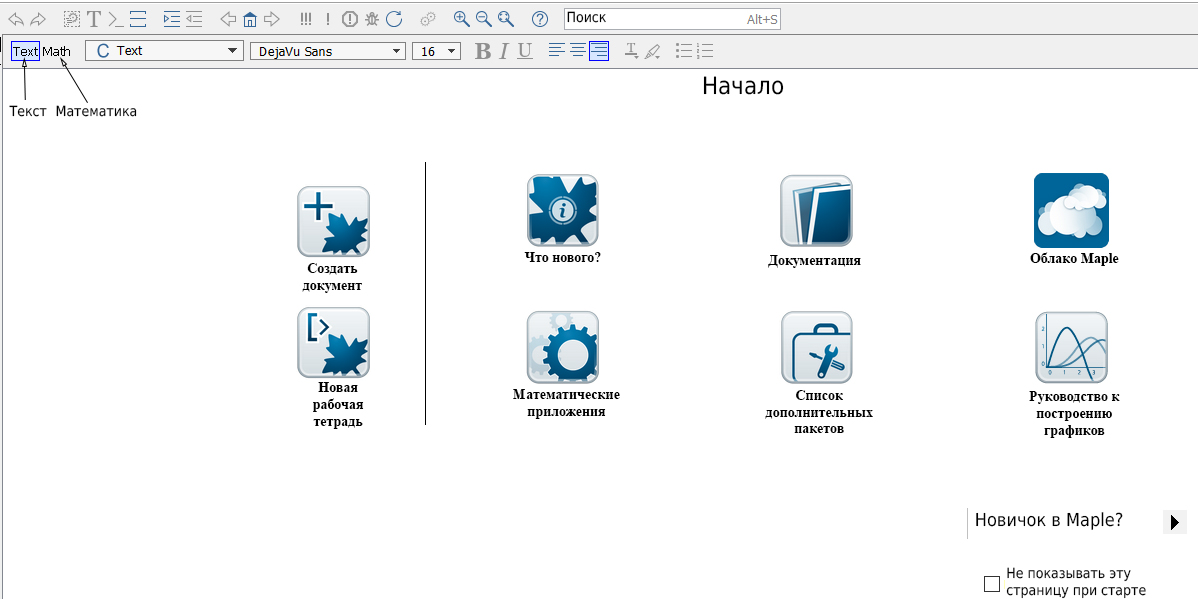
\includegraphics[width=.8\linewidth]{window-main}
        \caption{Главное окно программы Maple}
        \label{fig:window-main}
    \end{figure}
    \begin{figure}[H]
        \centering
        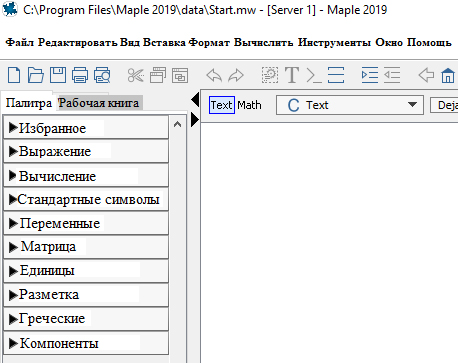
\includegraphics[width=.4\linewidth]{window-layout}
        \caption{Меню рабочей тетради}
        \label{fig:window-layout}
    \end{figure}
    \begin{figure}[H]
        \centering
        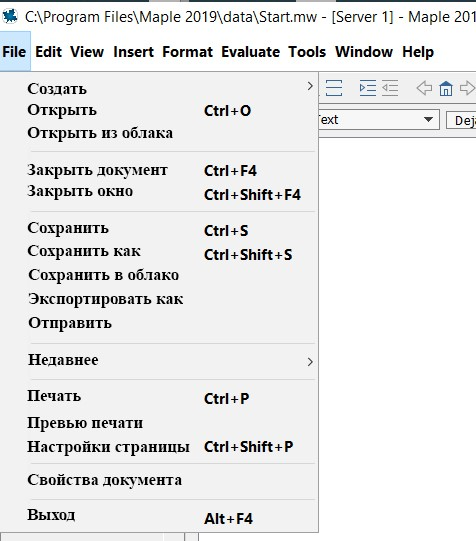
\includegraphics[width=.4\linewidth]{file}
        \caption{Меню команд файл}
        \label{fig:file}
    \end{figure}

    \section{Примеры программ в Maple}
    
    \subsection{Операции с формулами}
    Для демонстрации операций с формулами была написана следующая программа:
    \begin{lstlisting}
        rex := ((cos(x)^3 + sin(x)^4 + 2*cos(x)^4) - 2*sin(x)^4) - cos(2*x));

        упрощение:
        simplify(rex);
                               
        раскрытие скобок и факторизация:
        expand((x + 3)*(x - y));
        expand((x + 3)*(x + 1));
        w2 := % / %%;
        w2 := factor(w2);

        подстановка одного выражения в другое;
        subs(x = 500, w2);

        выделение левой и правой частей уравнений:
        y = a * x^2 + b;
        rhs(%);
        lhs(%%);
    \end{lstlisting}

    \subsection{Операции с полиномами}
    Для демонстрации операций с полиномами была написана следующая программа:
    \begin{lstlisting}
        pol := expand((5*x^2*y + x + 1)*(x^3 - x) + 2*y*x^2 + 6));
        
        целая часть от деления полиномов:
        quo(pol, x^3 - x, x);

        остаток от деления полиномов:
        os:rem(pol, x^3 - x, x);

        наибольший общий делитель двух полиномов:
        gcd(os, y*x^2+3);

        группировка:
        collect(pol, x);

        подстановка:
        pol1:=subs(y=2, pol);

        определение коэффициентов, дискриминанта, степени полинома:
        coeffs(pol1, x); discrim(pol1, x); degree(pol1, x);
    \end{lstlisting}

    \subsection{Ограничения на переменные}
    Для демонстрации ограничения на переменные была написана следующая программа:
    \begin{lstlisting}
        assume(n, integer); 
        cos(n*Pi);

        результат:
        (-1)^n
    \end{lstlisting}

    \subsection{Примеры математического анализа}
    Была написана следующая программа:
    \begin{lstlisting}
        f(x) := (x^3 - 3*x^2 + 2*x - 5)/(x^2 + 2):
        r:=5*sin((3*x)/(x-Pi)):

        вычисление пределов:
        limit(f(x), x = -1);
        limit(r, x = Pi);

        график функции r(x) := 5*sin((3*x)/(x-Pi)):
        plot(r, x=Pi-0.3..Pi+0.3);

        односторонние пределы:
        g(x) := 1/x:
        limit(g(x), x = 0, left);

        пределы функций нескольких аргументов:
        limit(x+1/y, {x=0, y=infinity});

        дифференцирование функции:
        f(x):=ln(sqrt(exp(3*x)/(1 + exp(3*x))));
        simplify(diff(f(x), x));

        частные производные:
        diff(f(x, y), x, y);

        производные высоких порядков:
        Diff(sin(x), x $ 3) = diff(sin(x), x $ 3);

        интегралы:
        Int((3*x^2 + 8)/(x^3 + 4*x^2 + 4*x), x) = int((3*x^2 + 8)/(x^3 + 4*x^2 + 4*x), x);

        определенный интеграл:
        Int(sin(phi)^3*sqrt(cos(phi)), phi=0..Pi/2)=int(sin(phi)^3*sqrt(cos(phi)), phi=0..Pi/2);

        несобственный интеграл:
        Int(1/(x^2+2*x+2), x= - infinity..infinity)= int(1/(x^2+2*x+2), x= - infinity..infinity);

        предел сходимости ряда:
        sum(7^(3*n)/(2*n - 5)!, n = 3 .. infnity) = evalf(sum(7^(3*n)/(2*n - 5)!, n = 3 .. infnity));

        произведение:
        product(a[k], k = 0 .. n);

        кусочно-аналитические функции:
        p:=piecewise(x<0, -1, x>1, 2*x, x^2);
        plot(p);
        int(p, x);
        dsolve({diff(y(x), x)+p*y(x), y(o)= -2}, y(x));
    \end{lstlisting}

    \subsection{Дифференциальные преобразования}
    Демонстрационная программа:
    \begin{lstlisting}
        Стандартное преобразование Лапласа:
        laplace(t^3+cos(t)=y(t), t, s);

        обратное преобразование Лапласа:
        invlaplace(%, s, t);

        тригонометрическое преобразование Фурье:
        fouriercos(1/(t^2 + 3), t, s);
    \end{lstlisting}

    \section{Описание библиотеки GF (Поля Галуа)}
    Пакет содержит только одну команду \code{GF(p, k, a)}, где:
    \begin{itemize}
        \item \code{p} - простое число;
        \item \code{k} - положительное число;
        \item \code{a} - (необязательный) неприводимый полином степени \code{k} над полем
              целых чисел по модулю \code{p}.
    \end{itemize}

    Команда GF возвращает таблицу G функций и констант для выполнения
    арифметических операций над конечным полем \code{GF(p\textsuperscript{k})},
    то есть полем Галуа c \code{p\textsuperscript{k}} элементами. Поле
    \code{GF(p\textsuperscript{k})} определено расширением \code{GF(p)[x]/(a)},
    где \code{a} -- неприводимый полином степени k над полем целых чисел по модулю \code{p}.

    Если \code{a} не указан, неприводимый полином степени \code{k} над полем целых чисел
    по модулю \code{p} выбирается случайным образом. К нему можно получить доступ как к
    константе \code{G:-extension}. Элементы \code{p\textsuperscript{k}} оторбражены в виде
    \code{modp1}.

    Для начала требуется объявить экземпляр используемого поля Галуа, например, \code{G:=GF(p\textasciicircum k)}.
    Это определит поле \code{G} с 8 элементами и все операции над ним.

    \section*{Выводы}
    В ходе лаборатоной работы было получено общее представление о математическом пакете Maple.
    Он позволяет решать математичские задачи аналитически и численно в удобном виде.
    В пакете присутствует множество типов данных, как стандартных для программирования,
    так и созданных для возможности аналитического решения задач, например натуральные дроби.

    Язык Maple кажется сложным из-за малоговорящих названий функций и их параметров,
    из-за чего приходится часто обращаться к документации. Кроме того, в некоторых
    случаях отсутствует унифицированное представление операций, например \code{D - diff}
    для дифференцирования.

    Работу в рабочей тетради Maple я нахожу неудобной т.к. текстовые стили работают
    в пределах одной строки и, соответственно, сбрасываются на следующей. 

\end{document}